\chapter{Background \& Objectives}

%This section should pick-up material from your progress report and enhance it based on the feedback and also your additional experience up to now. 

This section outlines the background of this project, mainly focusing on how the project came to
be and why it is an interesting topic to research into, as well as discussing some of the 
interdisciplinary work performed with art historians.

Carrying on from this, further sections detail some of the existing work that has already been 
performed on digital images of artwork and other methods which are useful in the context of this
project.

The main objectives and goals of this project are defined in the final sections and begin to
outline some of the analysis and classification techniques which are used in the project.

\section{Sir John Kyffin Williams}

Sir John Kyffin Williams (1918-2006) was one of the predominant figures in Welsh art of the
twentieth century.  He was advised by a doctor in the British Army to take up something which
would not tax his brain, such as painting, after failing a medical exam due to epilepsy. Kyffin --
as he was almost universally known in Wales -- studied at the Slade School of Art and worked as an
art master at Highgate School, before returning to live on his native Anglesey in 1973.  He was a
prolific painter and once claimed to have painted ``two pictures per week when in London, and 
three per week when in Wales.'\cite[p.209]{Williams1993Across} With a career spanning from the 
mid-1940s to approximately 2004, this rate amounts to a large body of work.

His style evolved from a very representational style to something more
expressive, which retained representational qualities: computer scientists
would say that the paintings became more \emph{blocky}; whilst art
historians say that his landscapes are almost constructed with swathes of textural
paint. His was a style characterised by thick impasto paint, applied almost
exclusively with palette knife, although the application technique appears to
change over time. This development of style led to the question: ``is it possible to
date the pictures from images alone?''

\begin{figure}[h]
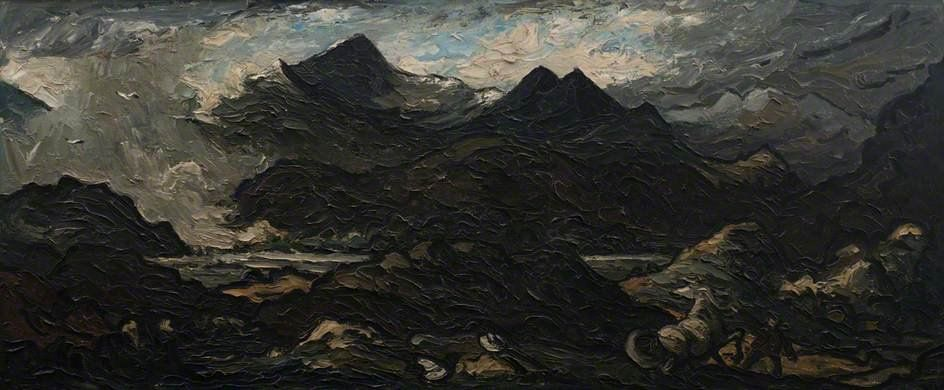
\includegraphics[width=\linewidth]{img/snowdon_horse.jpeg}
\caption[``\emph{Snowdon, the Traeth and the Frightened Horse}'']{``\emph{Snowdon, the Traeth and the Frightened Horse}'', Sir John Kyffin Williams, 1948: note curved strokes, rather than blocky application}\label{early_example}
\end{figure}


%\section{Background}
% 1 Page on Lloyd's work

Although also a portrait painter, Williams is primarily known for his landscape
paintings of north west Wales and Anglesey. While his technique and style
changed over the years, his landscapes in oil are instantly recognisable, often
featuring bold chunks of colour, and various points during his career bold
black outlines to figures and landscapes features. Greens, browns and greys
often form the palette of his paintings of the Welsh landscape. These colour
selections seem appropriate for the artist’s claim that melancholy, derived
from the ``dark hills, heavy clouds and enveloping sea mists'', is a national
characteristic of the Welsh.\cite{Williams1993Across} This combination of
colour selection and technique seems appropriate for the depiction of the areas
where he painted. Many of his most successful paintings are said to have a
``dark quality'' in depicting ``rain lashed hillsides,'' and it was this
darkness which ``makes his landscapes so distinctively
Welsh.''\cite{Davies2004100} 

\begin{figure}[h]
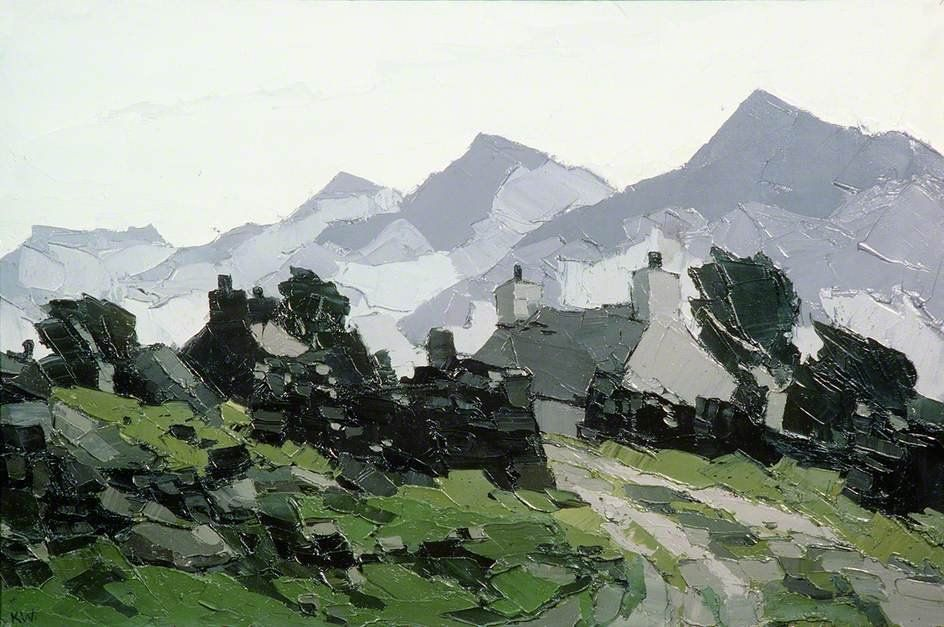
\includegraphics[width=\linewidth]{img/above_carneddi_no_2.jpeg}
\caption[``\emph{Above Carneddi, No. 2}'']{``\emph{Above Carneddi, No. 2}'', Sir John Kyffin Williams 1985: note much
blockier style and changed use of colour}\label{late_example}
\end{figure}

As his life progressed Williams's epilepsy grew steadily worse, especially when exposed to 
bright light. As a result most of his paintings are of overcast Welsh landscapes and appear to 
become visibly darker over time\cite{Harris2011How}.

%Both of the above descriptions could be applicable
%to paintings in the collections of the National Library of Wales such as
%Snowdonian Summits (1970-1990) or Yr Wyddfa a Grib Goch (1950-1960).

The aesthetic of Williams's Welsh landscapes is contrasted by the paintings he
made following a trip to Patagonia to paint the landscape and people of the
Welsh communities there in 1968 as part of a Winston Churchill Foundation
scholarship. The colours and application of paint in pictures produced in
following this journey (such as \emph{Lle Cul} (Figure~\ref{fig:lle-cul}), \emph{Henry Roberts},
\emph{Bryngwyn Patagonia}, \emph{Euros Hughes Irrigating his Fields}, all 1969,
National Library of Wales) differ starkly from paintings of Welsh landscapes,
incorporating pinks, purples and oranges. This contrast, combined with the fact
that the Patagonian pictures were produced during a definite period of time has
reinforced our interest in the analysis of the formal qualities of pictures
from different collections remotely, using digital images. 

\begin{figure}[h]
\centering
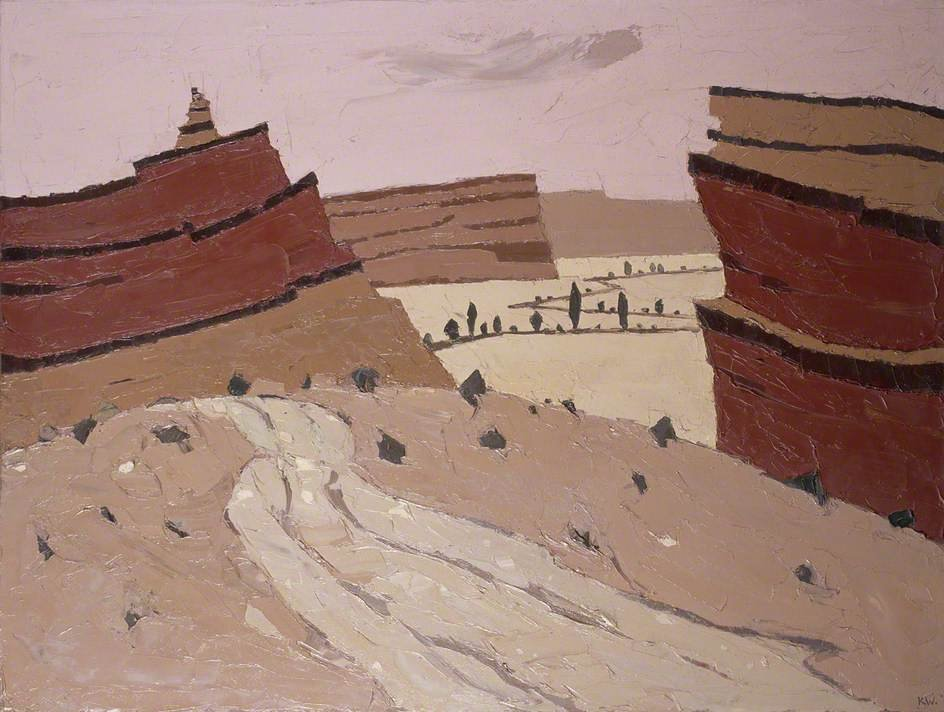
\includegraphics[width=0.75\textwidth]{img/lle-cul.jpg}
\caption[``\emph{Lle Cul, Patagonia}'']{``\emph{Lle Cul, Patagonia}'', Sir John Kyffin Williams 1969}
\label{fig:lle-cul}
\end{figure}

Williams's work is well represented in public collections in Wales
(particularly at the National Library of Wales, the National Museums and
Galleries of Wales and Oriel Ynys M\^{o}n, Anglesey). His pictures, often
depicting the landscape and people of north-west Wales were also tremendously
popular with the art buying public. Of the 325 paintings by Williams in public
collections in the UK listed on the BBC/Public Catalogue Foundation's ``Your
Paintings'' website, 212 of them are in the collections of the National Library
of Wales\cite{2013Your}. Many of these paintings were bequeathed to the Library
as part of a larger bequest by the artist (including works on paper and other
archival material). Many of the pictures which came to the library from the
artist's studio had little in the way of meta-data, and as such have been
catalogued with large date-ranges estimating the dates of production.  This
uncertainty in meta-data is another motivating force behind the current project.


\subsection{Taking a digital humanities approach to art history}

Digital humanities is an established area of research that brings together
digital content, tools and methods in order to address and create new knowledge
across the disciplines. Digital humanities approaches can be seen in two
distinct types of inquiry. The first is to carry out \emph{traditional}
humanities research more effectively or efficiently, by applying computational
methods or approaches to digitized humanities sources (originally text, image,
or audio-visual content from archives or libraries). Using John Unsworth’s
definition of ``scholarly primitives''\cite{Unsworth2000Scholarly} digital humanities
scholarship customarily involves the use of digital tools and methods for
discovering, annotating, comparing, referring, sampling, illustrating, or
representing humanities data. A classic example of this sort of work would be
the use of concordances and other computer-based analysis of digitized primary
sources that have been processed by optical character recognition software to
count, classify, or interpret digital texts (see, for example, the Historical
Concordance of the Welsh language\cite{2004Corpws}).  The second strand
of digital humanities inquiry is the development of new research questions that
can only be developed through the synthesis of digital content, tools and
methods: work that would have otherwise been unimaginable\cite{Hughes2011Evaluating}. This
type of research is by necessity multi-disciplinary, drawing together expertise
to be found across humanities, scientific and engineering disciplines, as well
as involving content experts from libraries, archives and museums. However, in
order to be truly transformative, this type of research must also be
interdisciplinary. 

The National Library of Wales now has a research programme in digital
collections, which is a forum for investigation into the digital collections of
Wales in collaboration with academics and students at universities in Wales and
beyond, in order to develop new research based around the digital content
created by the Library \cite{2012Research}. The research project described in this
article is an example of a digital humanities collaborative venture, bringing
together digital humanists, art historians, and computer scientists.  The
results of this research have value across all these groups. Arts historians
are able to better investigate a large corpus of digital paintings through the
application of computer science approaches to this content, and computer
scientists are able to configure new approaches in imaging to working with a
complex humanities dataset.

\section{Interdisciplinary work with the National Library of Wales}

This project originated through conversations between Hannah Dee and Gareth Lloyd Roderick on the
topic of the digital image processing of art; this led to Hannah building a small application to
show a Gaussian mixture model of Williams' work with the ultimate intention of being able to geographically
determine the location of a picture, especially those with a well defined setting especially those
painted at Crib Goch, a good example of which is shown in Figure~\ref{fig:crib-goch}.

\begin{figure}[h]
\centering
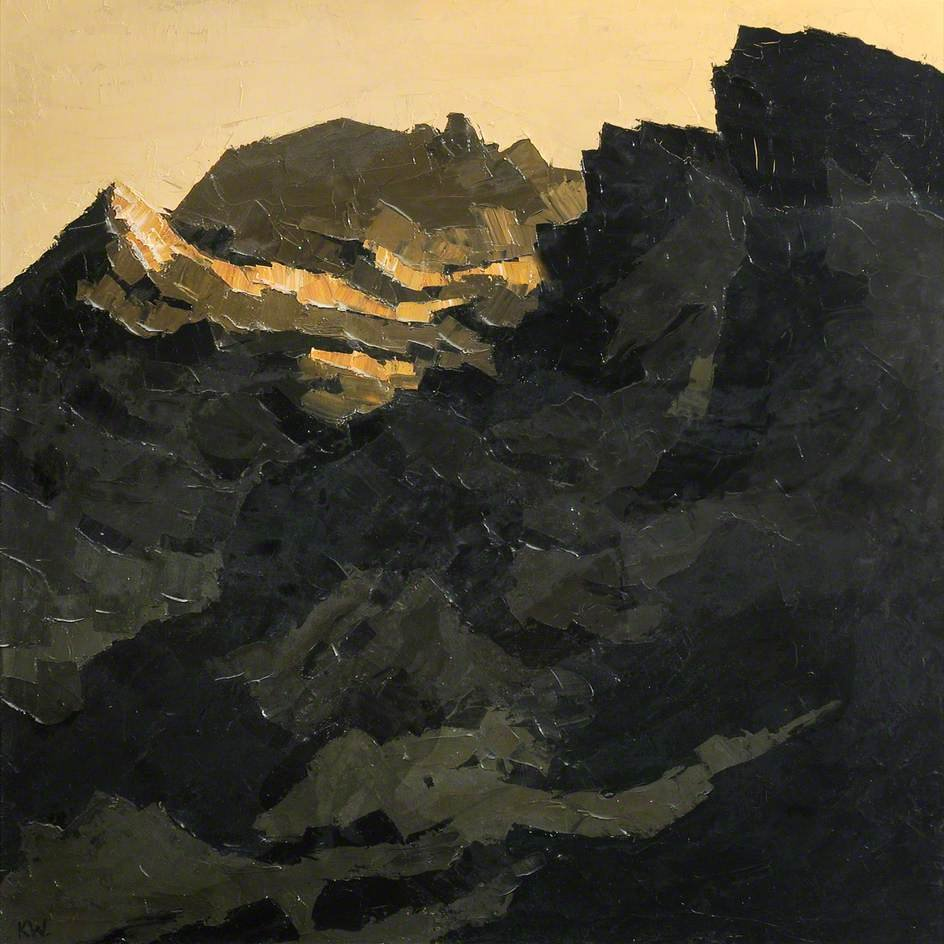
\includegraphics[width=0.75\textwidth]{img/crib_goch.jpg}
\caption[``\emph{Crib Goch}'']{``\emph{Crib Goch}'', Sir John Kyffin Williams}\label{fig:crib-goch}
\end{figure}

As has been discussed already, it becomes very clear to the human eye that Williams' style changes
dramatically as time progresses and, whilst it would be interesting to try and compare painted 
images to photographs of locations, the feasibility of being able to do so, especially given that
artists tend not to remain brilliantly faithful to the subject of their painting, is just so low
that it would have been very difficult to get any meaningful results. This makes temporal 
classification a much more appealing subject to research into.

To help with this Lloyd had produced a spreadsheet of all Williams' work known to the \gls{nlw}, 
including several collections over the country, but with the majority coming from the \gls{nlw}
collection. It was a part of Williams' will that the contents of his workshop was to be donated
to \gls{nlw} on the condition that any destroyed or defaced work was not to be displayed publicly.

Therefore this spreadsheet is the most comprehensive documents on Williams' work. Unfortunately a
lot of Williams' work does not have a lot of information on the dates in which it was painted, 
Llyod had made some good attempts at predicting the year based on when the painting first appeared
in exhibitions, so not all paintings have a single year associated with them. This spreadsheet 
does contain a lot of other useful meta-data as well as the year or year range in which the work 
was created, including canvas size and painting type. Not all of this meta-data was useful or 
relevant to temporal analysis, but is useful to the general study of Williams' work.

\subsection{Meetings with members of the National Library of Wales}

There have been two meetings to discuss the interdisciplinary work with members the National 
Library of Wales as well as a tour around the stores to view the \gls{nlw} collection of Williams'
work.


\subsubsection{Meeting of the 31\textsuperscript{st} October, 2011}
This meeting was between Lloyd, Hannah and I to discuss the state of the project particularly the
aims Hannah and I had for the project and when Lloyd's expectations and aspirations for the joint
work. Notably both our aspirations included being able to publish a paper before the submission of
the project, or, failing that, over the summer following the submission of the project.

This also provided an opportunity to discuss some of the artistic details with a more 
knowledgeable source which helped with the implementation of certain analysis techniques as well
as discussing more elements of Williams' life.


\subsubsection{Meeting of the 18\textsuperscript{th} February, 2012}
This meeting was between Lloyd, Hannah, Lorna M. Hughes\footnote{Lloyd's PhD supervisor} and I, again to discuss
the state of the project, but was also used to discuss finer details of the potential of 
publishing a paper. Lloyd was also able to provide a cleaner version of his spreadsheet.

More artistic details were discussed in the meeting, particular retaining to the application of
expert knowledge to the temporal classification of Williams' work. It was shortly after this 
meeting that Dr. Paul Joyner was contacted to provided artistic exemplars for many years in 
Williams' career.

Some other interesting and useful points were brought up with regards to Williams' work; such as the artistic cut-off 
point between early and late in Williams' career is around 1973. The theory that the canvas size
would be proportional to the year it was painted in due to the expense of paint on larger 
canvases.

It was also mentioned that the validity of some dates may be dubious, it might be the case that 
certain painting were said to be painted later than they actually were to increase the sale price.


\section{Existing Work}

\subsection{Edge-Orientated Gradients}\label{sec:existing-hogs}
As Williams's work is highly texturally, looking at the edge orientation of the image is
likely to be a valuable technique to use.

One technique recommended by Hannah was to look at \gls{hog}. The suggested paper outlined the use
of grids of \gls{hog} descriptors to improve the feature set for robust visual object
recognition\cite{Dalal2005Histograms}. As it significantly improves the feature set it seems
sensible to try and implement it as a technique to experiment with a non-colour-based approach.

The approach involves quite a few separate steps, only some of which are relevant to the project:

\begin{enumerate}
\item Gamma and colour normalization. Grayscale, \gls{rgb} and \gls{lab} spaces were used.
\gls{rgb} and \gls{lab} give similar results. Grayscale reduced performance less that square root 
gamma compression, but not as much as log compression.

\item Compute gradients. Often the simplest are the better here; Gaussian smoothing followed by 
discrete derivative masks (e.g.: Figure~\ref{fig:1x2-ddm}, Figure~\ref{fig:1x3-ddm}), etc. For 
colour this was done for each channel, and take the one with the largest norm.

\item Spatial and Orientation binning:
\begin{itemize}
\item Spatial binning is done by splitting the images into cells which can be rectangle or radial.
\item Orientation binning are spaced equally between either 0-180 "unsigned" or 0-360 "signed" 
bins.
\end{itemize}

\item Normalisation and Descriptor Blocks. Gradients vary over foreground/background, etc. 
Typically the blocks were overlapped so that each scalar response contains several components.

\item Pass a detector window across the image.

\item Run through a Linear \gls{svm} to classify the image.
\end{enumerate}

\begin{figure}[h]
$$
\begin{bmatrix}
-1 \\
1
\end{bmatrix}
$$
\caption{Example of a 1 by 2 Discrete Derivative Mask} \label{fig:1x2-ddm}
\end{figure}

\begin{figure}[h]
$$
\begin{bmatrix}
-1 \\
0 \\
1
\end{bmatrix}
$$
\caption{Example of a 1 by 3 Discrete Derivative Mask} \label{fig:1x3-ddm}
\end{figure}

Obviously, when applying this as an analysis technique to paintings, there are some points which
are completely irrelevant. Passing a detector window and running through a Linear \gls{svm} are
the obvious two. Normalisation is another unneeded step as time complexity isn't a problem which
needs to be thoroughly considered, as long as the analysis completes within a reasonable amount of
time.

The leaves the act of computing the gradients (again, this can be done without Gaussian smoothing
as that reduces accuracy) which should a simple matter implemented by earlier techniques. Binning 
by \gls{rhog} or \gls{chog} descriptors, which may prove to the one of the more difficult parts of
implementing this technique.

\Gls{rhog} descriptors have similarities to \gls{sift} descriptors, but are used quite 
differently; \gls{sift} descriptors are optimised for sparse baseline matching whilst \gls{rhog}
descriptors are optimised for the dense and robust coding of a spatial form. The size of the
descriptor affects performance when using \gls{rhog}, for paintings it may turn out that a size
relating to the original size of the painting is a good way of getting around this problem.

\Gls{chog} descriptors become more complex still. They are similar to Shape 
Context\cite{ Belongie2001Matching}, but differ in one key aspect: in \gls{chog} descriptors each
spatial cell holds a stack of gradient-weighted orientation cells over an orientation-independent
edge-presence count which Shape Contexts use.

According to the author it is better to think of \gls{chog} descriptors as an advanced form of 
centre-surround coding as small descriptors with very few radial bins gave the best results.

Local contrast normalisation can be performed to help against local variations in the illumination
of foreground and background.

It would seem that both \gls{rhog} and \gls{chog} descriptors are designed more for the detection
window rather than analysis technique. This may make them less useful and result in an implemented
technique being just a simple histogram of edge orientations.

\subsection{Brush-stroke Analysis}\label{sec:existing-brush-stroke}
Stroke analysis is one of the main goals for this project. It is quite apparent from looking at 
Williams's paintings that his brush-strokes change over time, his early work having lots of
smaller strokes over the canvas to large bold strokes in his later work.

The first paper found relating to the analysis of brush-strokes involved moving a circular filter
across the whole painting to find the ridges of strokes, then filling any unbroken areas. They then
shrunk these areas to a single pixel line and fitted a $n^{\text{th}}$ order polynomial to this
line\cite{Berezhnoy2005Authentic}. This method seems fairly simplistic, but could be an interesting
first step, but as it is more focused on authenticating paintings it may be of limited use.

Another method for stroke analysis has been published in the IEEE Transactions on Pattern Analysis
and Machine Learning journal. This method is far more complex, but is able to extract and label
individual brush-strokes. An interesting part of their findings was the ability to date some of Van
Gogh's paintings to a known period in his career\cite{Li2012Rhythmic}.

This method involves performing edge detection of the painting followed by an edge linking 
algorithm which aims to remove small, noisy edges and to trace every edge. With this they then
perform enclosing, as strokes may not be complete this stage also aims to fill in missing gaps of
strokes and to fill these in within a certain tolerance.

The algorithm then decides if a stroke really is a painted stroke, if the stroke is completely 
enclosed, isolated from other non-edge pixels and forms a connected component then it is likely 
that it is a proper brush-stroke and is extracted. The edge pixels are used as the background and
the non-edge pixels as the foreground, this is the process of labelling the brush-stroke.

For each of these labelled candidates, a heuristic function is used to threshold any brush-strokes 
that are either too long or too short, these strokes are discarded. These strokes are then
considered to be candidates if they are not significantly branched, the stroke is not too wide 
(this may change for Williams as he used a pallet knife rather than a brush) and the 
brush-stroke is not too big or small.

Separately, the image is then segmented using $k$-means clustering by \gls{rgb} values. This clustering 
algorithm is applied several times, lowering the tolerances for distance within a cluster. 
Connected components as a result of this clustering and have noise reduction performed upon them.
Finally, the two types of brush-strokes are combined.

This technique may need some changing to account for Williams's use of a pallet knife, but
the overall principals of this technique should work with Williams's paintings.


\section{Analysis Objectives}
Analysis is one of the biggest sections of this project and involves creating techniques which 
will allow comparison of paintings in a way which will allow some form of classification to be
performed on them.

Typically it is expected that this produces some form of high-dimension state space in which each
painting is a point in the state space. From this state space the distance between one painting
and another can be easily resolved using a distance measure like Manhattan distance 
\eqref{eq:manhattan_distance}, euclidean distance \eqref{eq:euclidean_distance} or a distance 
measure more specific to the state space should it be needed (e.g.: chi-squared for histograms).

\begin{equation}\label{eq:manhattan_distance}
d_1(\mathbf{p},\mathbf{q}) = \|\mathbf{p}-\mathbf{q}\|_1 = \sum^{n}_{i=0}{|p_i-q_i|}
\end{equation}

\begin{equation}\label{eq:euclidean_distance}
d(\mathbf{p}, \mathbf{q}) = \sqrt{\sum^{n}_{i=0}({q_i-p_i})^2}
\end{equation}

\subsection{Colour-space Analysis}
The simplest way of analysing a digital image is to look at the colours which it consists of.
Doing this is relatively simple; each pixel has a set of values defining the colour of that point,
getting something meaningful from this is less simple.

The simplest strategy is to perform some form of statistical analysis on each painting then use
this for classification. Several good and computationally cheap options exist for this; 
mean \eqref{eq:mean} and standard deviation \eqref{eq:std_dev}, are some good
examples which often come predefined in image processing and computer vision libraries.

\begin{equation}\label{eq:mean}
\upmu = \frac{1}{N}\sum_{i=1}^{N}x_i
\end{equation}

\begin{equation}\label{eq:std_dev}
\sigma = \sqrt{\frac{1}{N}\sum_{i=1}^{N}(x_i - \upmu)^2}
\end{equation}

The representation of colour is another important factor, an \gls{rgb} representation will have all 
three values change if there are many changes in brightness of the colours whilst a \gls{hsv} 
representation will only have a single value change.

Therefore, an object of this section should be to explore different colour models and statistical
methods which can be applied to them.

Another useful technique which should be investigated early into the project are image histograms.
These histograms plot the distribution of colour across an image and are therefore a very powerful
method of analysing an image, especially for comparison. As with statistical analysis, histograms
will be largely effective by colour model.

\subsection{Texture Analysis}
As Williams's work is very textural, it follows that a main part of the analysis should
focus around the texture of his paintings. Unfortunately for this section, it seems unlikely that
I will be able to get any 3-dimensional models of Williams's paintings. This would have been a nice,
if rather large, section of the project.

Instead it is more sensible to look at the orientation of edges in Williams's work. Some useful 
pre-existing techniques have already been discussed in section~\ref{sec:existing-hogs}. Histograms
of edge orientation\cite{Dalal2005Histograms} seem like a promising concept which may prove 
relatively simple to implement.

This section may also help with any work into brush-stroke analysis (see 
section~\ref{sec:analysis-brush-stroke}).

\subsection{Brush-stroke Analysis}\label{sec:analysis-brush-stroke}
With Williams's distinctive style and how obviously this style changes over time, the ultimate aim 
of this project is to be able to analyse the brush-strokes\footnote{A slight misnomer as Williams 
used a palette knife to paint with rather than a traditional brush} in a painting.

From looking at the paintings it is very apparent that in his earlier work he made a lot more 
strokes than in his later works\footnote{Although this isn't quite true as the canvases he worked
on in his later life tended to be larger}. The strokes in his later work tend to have larger areas
and span more of the canvas.

If it is possible to calculate a rough amount and size of strokes made in a given painting it 
should be a reasonable piece of data to classify on. As previously discussed in section~
\ref{sec:existing-brush-stroke} there has already been a decent amount of research into determining
brush-strokes in a painting. 

It would be preferable to try and take one of the techniques discussed in that research and change
it to suit the needs of the project rather than attempting to create a whole new method of 
brush-stroke recognition.

\subsection{Ensemble Techniques}
With some of the aforementioned analysis techniques it makes sense to combine two or more 
techniques together; a good example would be colour histograms and histograms of edge orientation.

This form of analysis is inspired by the concept of the same name in statistics and machine 
learning which tend to obtain better predictive performance. It may also be worth while trying to
weight different techniques so that the techniques which give the best performance affect the 
result of the ensemble technique more.


\section{Classification Objectives}
The overall objective of classification is to be able to label a painting by Williams as 
being painted in a given year based on analysis performed on all other paintings with known years.

This ties in with the main aim of this project of being able to classify any Williams
painting, whether it has a known or unknown year, as being from a given year. Evidently for 
paintings with an unknown year it is difficult to know how accurately the system has been, so, for
the most part, these paintings have been ignored and those paintings with a known year have made
up the training and validation set.

This can be used to evaluate the performance of the analysis technique and classification 
algorithm. Pearson's product-moment correlation coefficient \eqref{eq:pearsons} between actual year
and classified year has been suggested to be a good performance measure for this project.

\begin{equation}\label{eq:pearsons}
\rho_{X,Y}={\mathrm{cov}(X,Y) \over \sigma_X \sigma_Y} ={E[(X-\mu_X)(Y-\mu_Y)] \over \sigma_X\sigma_Y}
\end{equation}


\subsection{Classification}
One of the simplest methods of classification is $k$-Nearest Neighbour from
this one can take a poll of the years for each neighbour and assign the year of the painting to
classify to be the average of these years.

Depending which form of average you take (mathematical mean, median or mode) will
alter the result; although it should be noted that median is very unlikely to give a result on its
own due to the sparseness of the data.

There are other techniques which could be applied to this problem, but the rewards for 
implementing them is not likely to be outweighed by the time it would take to implement such
techniques. There is a workaround for this; there are several machine learning tool-kits which 
provide pre-implemented version of these techniques.

One of the most popular tool-kits available for general use is Weka\cite{Hall2009WEKA}, which is discussed in more
detail in section~\ref{sec:bg-weka}.

% FIXME Find out who Julie is here.
Another technique suggested by Julie Greensmith is to use \gls{lcs}\cite{Bacardit2013Largescale}, 
which has an implementation for Weka. This may prove to give very good results for the kind of
analysis being performed on Williams's work.

\subsubsection{Use of Weka}\label{sec:bg-weka}
Weka is a machine learning toolkit which boasts an impressive number of learning techniques. As
such is makes sense to use it to help classify the results of analysis techniques. This does mean
adding additional logic to export data in a form Weka understands, but the results from Weka
may provide a new and detailed insight into our own analysis techniques which $k$-Nearest 
Neighbour cannot.

%\subsubsection{Learning Classifier Systems (LCS)}

\subsection{Exemplars}
Another method of classification is to incorporate expert knowledge, making use of the 
interdisciplinary work with members the \gls{nlw}, instead of a dataset as the ground truth for
the classification technique. This expert knowledge takes the form of a set of exemplar paintings
for each year in Williams' career and therefore also allows these exemplars to be compared to the
statistical centre of that year range to allow the comparison digital analysis to human experts.
